\documentclass[12pt]{book}

\usepackage[utf8]{inputenc}
\usepackage[spanish,es-tabla]{babel}
\parindent = 0cm

\usepackage{amsmath}
\usepackage{amssymb,amsfonts,latexsym,cancel}
\usepackage{graphicx}
\usepackage{float}
\usepackage{subfigure}
\usepackage{vmargin}
\usepackage[usenames,dvipsnames,svgnames,table]{xcolor}

\setpapersize{A4}
\setmargins{2.5cm} % margen izquierdo
{1.5cm}            % margen superior
{16.5cm}           % anchura del texto
{23.42cm}          % altura del texto
{10pt}             % altura de los encabezados
{1cm}              % espacio entre el texto y los encabezados
{0pt}              % altura del pie de página
{2cm}              % espacio entre el texto y el pie de página

\begin{document}

\title{
\begin{center}

\includegraphics[scale=1]{figuras/cartelfiuba.png}\\[3cm]
\end{center}
Circuitos Electrónicos II - 66.10\\ Trabajo Práctico Nº 2\\[2cm]
Análisis del amplificador de potencia del Turner 730\\[1cm]
\begin{flushleft}
Alumnos, Docentes
\end{flushleft}}
\author{}
\date{}
\maketitle
%\tableofcontents

\section{Objetivos}
\subsection{Resumen de objetivos}
ver
\subsection{Desarrollo}
ver

\newpage
\begin{figure}[!ht]
\centering
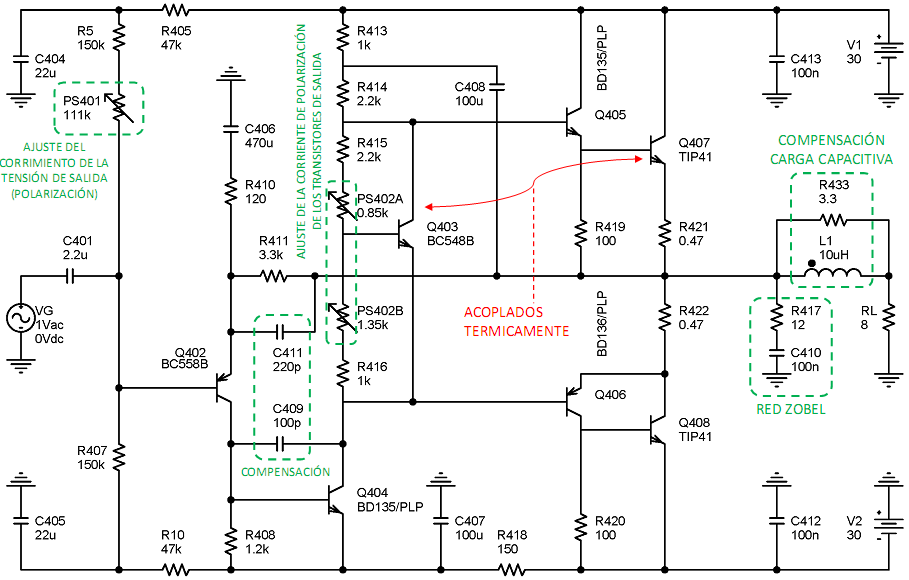
\includegraphics[scale=0.5]{figuras/CircuitoPropuesto.png}
\caption{Circuito a analizar y simular. REEMPLAZAR AGREGANDO ETAPAS}
\label{circuito}
\end{figure}

\newpage
\section{Desarrollo}
\subsection{Punto 1}
\textbf{Enunciado : } Calcular las tensiones de todos los nodos y las corrientes de todas la ramas para VG=0V\\[1cm]
\begin{figure}[H]
\centering
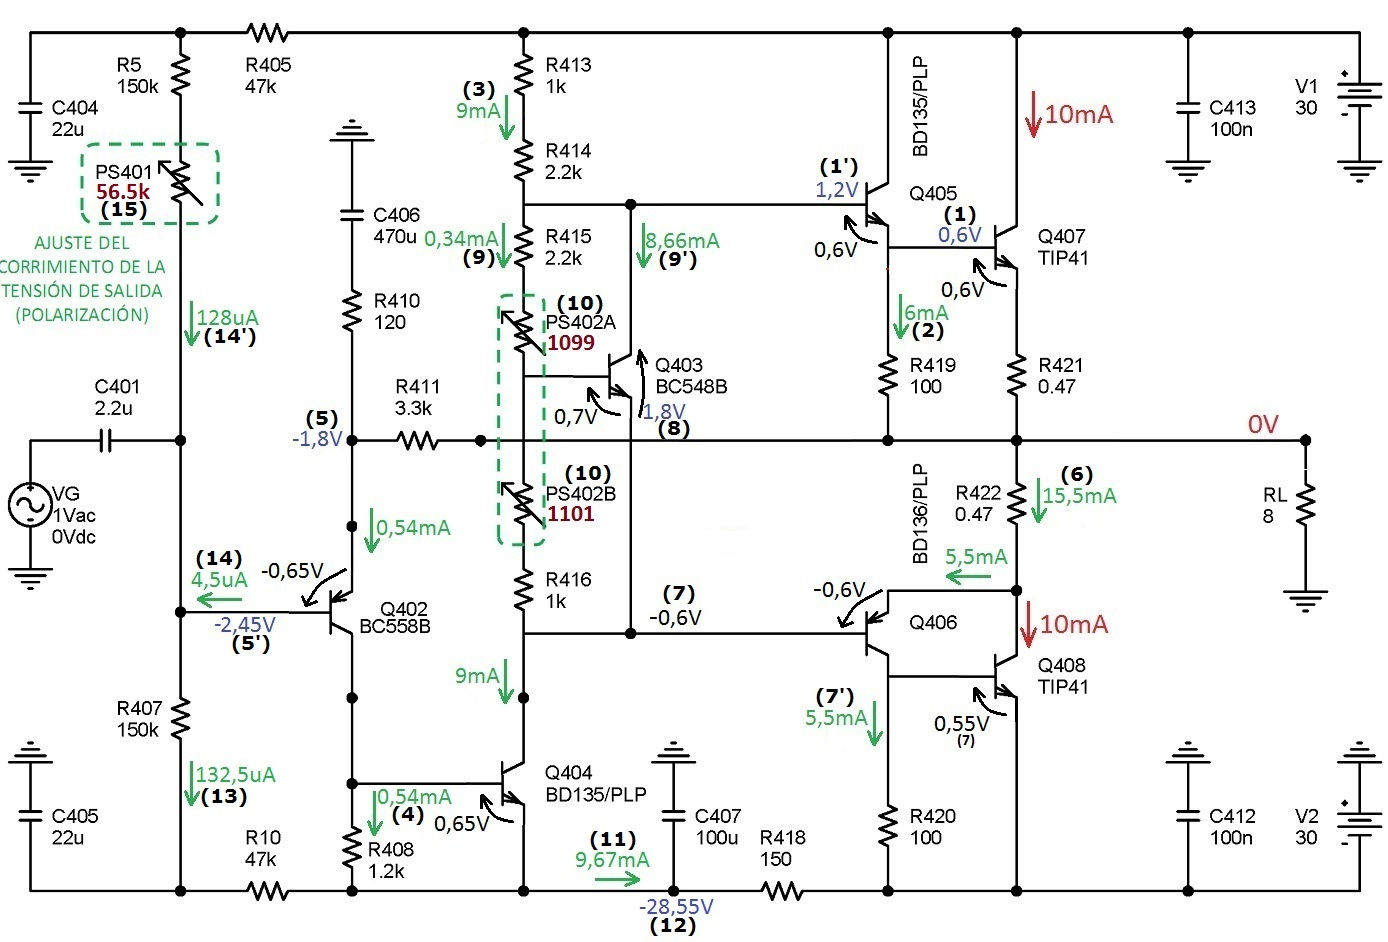
\includegraphics[scale=0.4]{figuras/1-valoresReposo.png}
\caption{Valores de polarización calculados}
\label{figura1}
\end{figure}
Los valores de $\beta$ como los de $V_{BE}$ se tomaron de las hojas de datos de los respectivos transistores, excepto la tensión de Early, $V_{A}$ , que fue tomada del modelo spice correspondiente.\\
Para $\beta$ de Q402/3 se tomó el valor típico, y para los restantes el promedio entre el máximo y el mínimo.\\

\begin{table}[H]
\centering
\begin{tabular}{|l|c|c|c|c|c|}
\hline
&$\beta$&$I_{CQ}$(mA)&$g_{m}$(mA/V)&$r_{\pi}$($\Omega$)&$r_{o}$($\Omega$)\\
\hline
Q402&330&0,54&21,6&15,3K&\\
\hline
Q403&330&8,66&346&954&\\
\hline
Q404&140&9&360&389&12,9K\\
\hline
Q405&140&6&240&583&\\
\hline
Q406&140&5,5&220&636&\\
\hline
Q407&50&10&400&125&\\
\hline
Q408&50&10&400&125&\\
\hline
\end{tabular}
\caption{Parámetros calculados para el punto de reposo.}
\label{Polarizacion}
\end{table}

Se procedió a tomar en cuenta primero los requisitos de salida $V_{OQ}$=0V e $I_{CQ407/8}$=10mA, se despreciaron todas las corrientes de base de los transistores (excepto $Q_{402}$, para ajustar PS401)\\
Se realizaron los siguientes pasos :
\begin{itemize}
\item (1) $V_{BQ407}$=0,6V , estimado de la Figura 10 ``On Voltages'' de la hoja de datos del transistor TIP41A-D.
\item (1') $I_{R419}=\dfrac{0,6V}{R419}=6mA$
\item (2)  $V_{BQ405}$=1,2V , a $V_{BQ407}$ se suma $V_{BEQ405}$=0,6V , este último estimado de la Figura 4 ``Base-Emitter On Voltage'', de la hoja de datos del transistor BD135-On, tomando la corriente obtenida en (1').
\item (3) $I_{CQ404}=\dfrac{30V-1,2V}{R413+R414}$=9mA
\item (4) $I_{CQ402}=\dfrac{V_{BEQ404}}{R408}$=0,54mA , donde $V_{BEQ404}$ se estima de la Figura 4 ``Base-Emitter On Voltage'', de la hoja de datos del transistor BD135-On, tomando la corriente obtenida en (3).
\item (5) $V_{EQ402}=Vo_Q-I_{CQ402}.R411=-1,8V$
\item (5') $V_{BQ402}$=$V_{EQ402}+V_{BEQ402}=-1,8V-0,65V=-2,45V$ , donde $V_{BEQ402}$ se estima de la Figura 2 ``Saturation and On Voltages'', de la hoja de datos del transitor BC558B-Motorola, usando la corriente obtenida en (4).
\item (6) $I_{R422}=I_{CQ407}+I_{R419}-I_{R411}$= 10mA + 6mA $-$ 0,5mA = 15,5mA.
\item (7) $V_{BQ408}$=0,55V , estimado de la Figura 10 ``On Voltages'' de la hoja de datos del transistor TIP41A-D, se elige menor que en (1) debido a que en este caso no tenemos resistencia de emisor y coincida con $I_{CQ406}$, que hallamos en el siguiente item.
\item (7') $I_{CQ406}=15,5mA-10mA=5,5mA$ , $V_{BQ406}=-0,6V$ , estimado de la Figura 4 ``Base-Emitter On Voltage'' de la hoja de datos del transistor BD136-On, usando $I_{CQ406}$, recién obtenida.
\item (8) $V_{CEQ403}=V_{CQ403}-V_{EQ403}=1,2V-(-0,6V)$= 1,8V.
\item (9) $I_{R415}=\dfrac{V_{CEQ403}}{R415+PS402+R416}=\dfrac{1,8V}{5,4K\Omega}$=0,33mA.
\item (9') $I_{CQ403}=I_{R414}-I_{R415}=9mA-0,33mA=8,67mA$
\item (10) Primeramente obtenemos $V_{BEQ403}$=0,7V de la Figura 2 ``Saturation and On Voltages'', de la hoja de datos del transitor BC548B-Motorola.\\
Luego tenemos que PS402B=$\dfrac{0,7V}{0,33mA}-1K\Omega=1121\Omega$.\\
Con lo que PS402A$=2200\Omega-1121\Omega=1079\Omega$
\begin{center}
PS402A=1079$\Omega$  y  PS402B=1121$\Omega$
\end{center}
\item (11) Primero se considera que solamente 9.54mA, la suma de $I_{CQ404}$ e $I_{R408}$, pasan por R418, con esto se obtuvo un primer valor de (12) de $-28,57V$, con esto ultimo se obtiene $I_{R407}=\dfrac{-2,45-(-28,57)}{197K\Omega}=132,6\mu A$, con esto obtenemos el valor final de (11) de 9,67mA.
\item (12) $V_{EQ404}=9,67mA . 150\Omega-30V=-28,55V$.
\item (13) Con este valor reajustamos $I_{R407}$ para ajustar mejor PS401, quedando finalmente  $I_{R407}=\dfrac{-2,45-(-28,55)}{197K\Omega}=132,5\mu A$.
\item (14) $I_{BQ402}=\dfrac{I_{CQ402}}{\beta_{402}}=\dfrac{0,54mA}{330}=1,6\mu A$.
\item (14') $I_{PS401}=I_{R407}-I_{BQ402}=130,9\mu A$.
\item (15) $PS401=\dfrac{30V-(-2,45V)}{130,9\mu A}=50,9K\Omega$
\end{itemize}

\subsection{Punto 2}
\textbf{Enunciado : } Calcular la ganancia de lazo para frecuencias medias (1KHz)\\[1cm]
Para este punto hacemos el esquemático para alterna, reemplazamos la tercera etapa por un bloque con ganancia de tensión unitaria, para mayor claridad.\\
\begin{figure}[H]
\centering
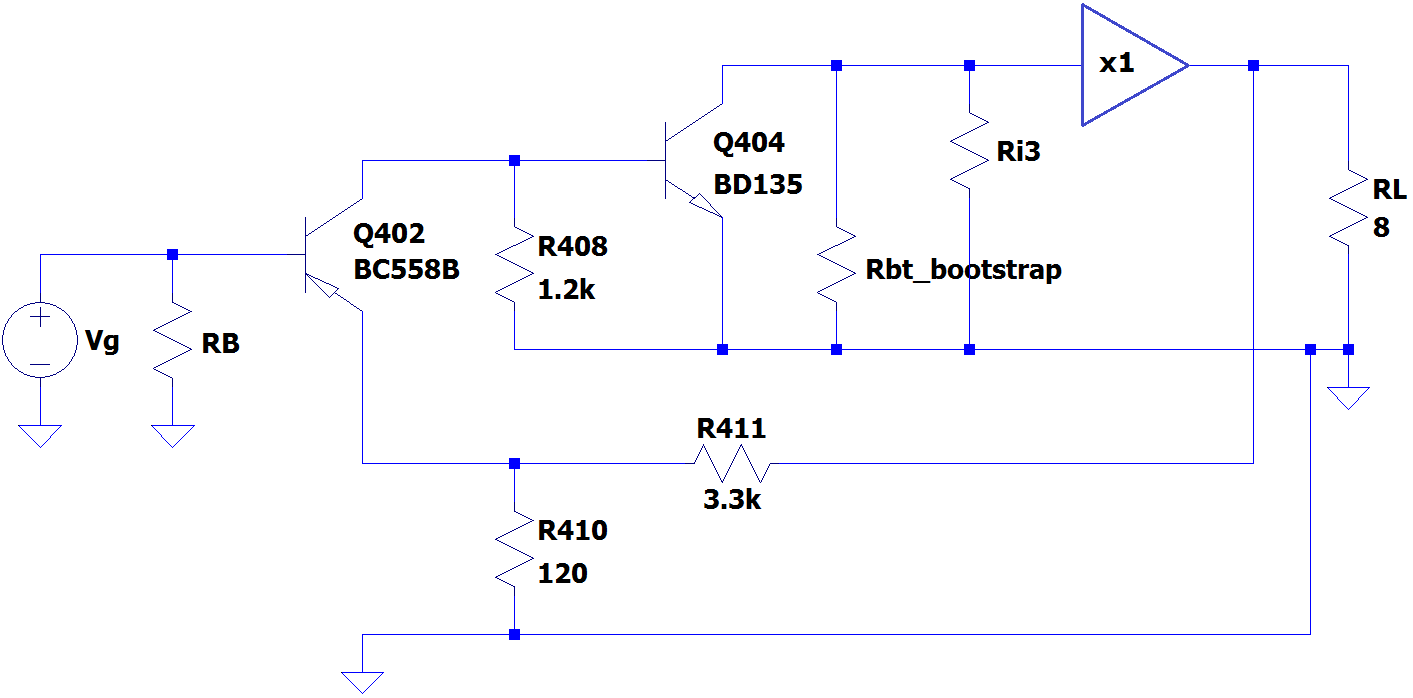
\includegraphics[scale=0.4]{figuras/2-lazoCerrado.png}
\caption{Realimentación Serie-Paralelo}
\label{figura2-1}
\end{figure}
Al muestrear tensión y sumar tensión tenemos que a la entrada se comparte la corriente y a la salida la tensión, entonces parametrizamos la realimentación con parámetros híbridos H.
\begin{center}
El factor de realimentación $f$ , es:\qquad $f$ = $h_{12}$ = $\dfrac{120\Omega}{120\Omega+3,3K\Omega}$ = 0,035
\end{center}
Luego $h_{11}$=R410//R411 se acopla a la entrada, y $h_{22}$=R410+R411 a la salida para considerar una realimentación ideal:
\begin{figure}[H]
\centering
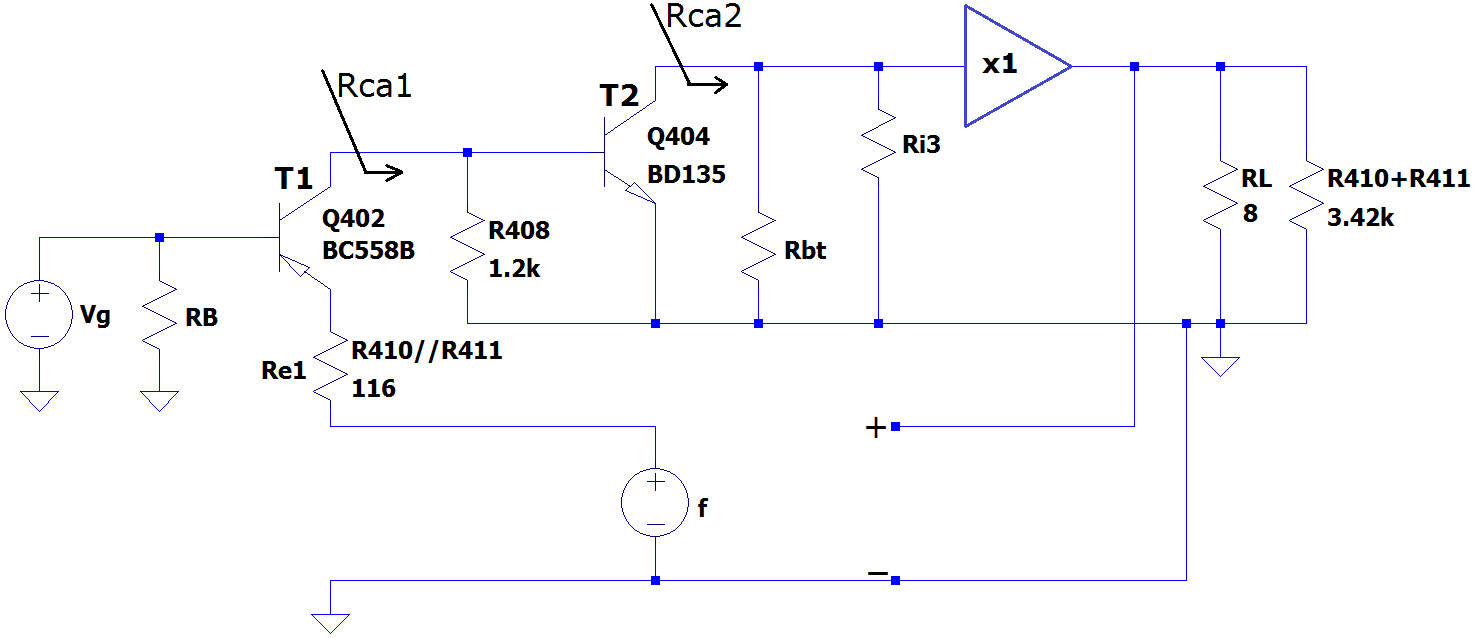
\includegraphics[scale=0.4]{figuras/2-lazoCerradoIdeal.png}
\caption{Realimentación Serie-Paralelo ideal}
\label{figura2-2}
\end{figure}
Se despreció $h_{21}$, el efecto de la salida sobre la entrada.\\[0.5cm]
$Av_{1} = \dfrac{-gm_{1}Rca1}{1+gm_{1} Re1} = \dfrac{-gm_{1}(R408//r_{\pi_2})}{1+gm_{1}(R411//R410)} = -1,81$\\
$Av_{2} = -gm_{2}Rca2 = -gm_{2}(ro_{2}//Ri_{3}//Rbt) = -360\dfrac{mA}{V} 10K\Omega = -3600$\\[0.5cm]
Donde :\\
Ri3 $=\beta_{405} \beta_{407} RL = 140$ . 50 . $8\Omega = 56K\Omega$\\
$ro_{2}$ = 12,9K$\Omega$ es la resistencia de salida correspondiente al modelo a $Q_{404}$\\
Rbt = 100 . R414 = 100 . 2,2K$\Omega$ = 220K$\Omega$ es la resistencia de bootstrap
\begin{center}
$\Longrightarrow$   Av = Av1 . Av2 . Av3 = (-1,81)(-3600) 0,99 = 6450,84\\
\end{center}
La ganancia del amplificador a lazo abierto es  $a$ = Av ($\dfrac{zc}{zc+ro}$) ($\dfrac{ri}{zg+ri+Re1}$)\\
Siendo :\\
$zc$ = RL//(R411+R410) = 7,98$\Omega$\\
$ro=ro_{sup}//ro_{inf}=2,92\Omega$\quad aproximada, debido a que al tratarse de una etapa clase AB, los transistores de potencia Q405/7 no están en conducción de alterna todo el ciclo.\\
.... $ro_{sup} = 0,47\Omega+\dfrac{r\pi_{407}}{\beta_{407}}+\dfrac{R419}{\beta_{407}}//\dfrac{r\pi_{405}}{\beta_{407}\beta_{405}}$ = 7$\Omega$\\
.... $ro_{inf}=0,47\Omega+\dfrac{r\pi_{406}}{\beta_{406}}=5\Omega$\\
$zg=0$, ya que la resistencia interna de la fuente es nula\\
$ri =r_{\pi_1}+\beta_{Q402} . R410=54,9K\Omega$\\
$Re1=R410//R411=116\Omega$
\begin{center}
$\Longrightarrow$   $a$ = 4712,77\\
\end{center}
Con lo que la ganancia a lazo abierto, T, es :
\begin{center}
T = $a$ $f$ = 164,9\\
\end{center}

\subsection{Punto 3}
\textbf{Enunciado : } Calcular la ganancia global para frecuencias medias (1KHz)\\
\begin{center}
Ganacia global\quad A = $\dfrac{a}{1+af}$ = 28,4
\end{center}
Que es aproximadamente igual a $\dfrac{1}{f}$, (28,6), debido a que $T$ es mucho mayor que 1.
\subsection{Punto 4}
\textbf{Enunciado : } Calcular la máxima potencia obtenible sobre la carga para frecuencias medias (1KHz)\\[1cm]
Máxima potencia disipada por el transistor $Q_{407/8}$:\quad $Pc_{max}=\dfrac{Vcc^{2}}{\pi^{2}RL}=11,4W$\\[0,75cm]
Que es el 40\% de la máxima potencia disipada en la carga $P_{cargamax}$, entonces :
\begin{center}
$P_{cargamax}$=28,5W
\end{center}

\subsection{Punto 5}
\textbf{Enunciado : } Calcular la impedancia de entrada para frecuencias medias (1KHz)\\[1cm]
Rin = [($1+af$) Rib]//Rb\\
Rib = ri+Re1 = 55K$\Omega$\\
Rb = (R5 + PS401) // R407 = 85,84K$\Omega$
\begin{center}
$\Longrightarrow$  Rin = 85K$\Omega$
\end{center}

\subsection{Punto 6}
\textbf{Enunciado : } Calcular la impedancia de salida para frecuencias medias (1KHz)\\[1cm]
$Ro=\dfrac{ro//RL//(R410+R411)}{1+af}$\quad al estar muestreando tensión.
\begin{center}
$\Longrightarrow$  Ro = 12,9m$\Omega$
\end{center}

\subsection{Punto 7}
\textbf{Enunciado : } Calcular el factor de amortiguamiento para frecuencias medias (1KHz)\\[1cm]

Factor de amortiguamiento, Df (Damping factor) :\qquad Df =$\dfrac{RL}{Ro}$\\
\begin{center}
$\Longrightarrow$  Df = $\dfrac{8\Omega}{12,9m\Omega}$ = 620
\end{center}
VER PAGINA 120, AudioPowerAmplifierDesignHandbook DOUGLAS SELF

\subsection{Punto 8}
\textbf{Enunciado : } Calcular la máxima tensión pico sobre la carga para frecuencias medias (1KHz)\\[1cm]
Vimos en el punto 4 que :\quad $P_{cargamax}$=28,5W\\[0.25cm]
Entonces\quad $V_{max}$ = 15,1V
\begin{center}
$\Longrightarrow$  $V_{picomax}$ = 21,3V
\end{center}

\subsection{Punto 9}
\textbf{Enunciado : } Calcular la máxima eficiencia obtenible con este amplificador para frecuencias medias (1KHz)\\[1cm]
Eficiencia máxima\quad $\eta_{max}=\dfrac{P_{cargamax}}{P_{fuente}}=\dfrac{\frac{Ip.Vp}{2}}{\frac{2 Ip.Vcc}{\pi}}$
\begin{center}
$\Longrightarrow$  $\eta_{max}$ = 55\%
\end{center}

\subsection{Punto 10}
\textbf{Determinar : }\\

\subsubsection{Punto 10.a)}
\textbf{Enunciado : } El tamaño de los disipadores para cada transistor (resistencia térmica disipador ambiente)\\[1cm]
Para los transistores de señal tenemos :
\begin{table}[H]
\centering
\begin{tabular}{|l|c|c|c|c|c|c|c|}
\hline
&Modelo&$I_{CQ}$(mA)&$V_{CEQ}$(V)&$P_{D}$(mW)&$P_{Dmax}$(mW)&$^{o}C/W$&$^{o}C/W$\\
\hline
Q402&BC558B&0,54&26,1&14,1&625&200&83,3\\
\hline
Q403&BC548B&8,66&1,8&15,6&625&200&83,3\\
\hline
Q404&BD135&9&27,95&251&1,25&100&10\\
\hline
Q405&BD135&6&29,4&81,4&1,25&100&10\\
\hline
Q406&BD136&5,5&29,4&81,4&1,25&100&10\\
\hline
\end{tabular}
\caption{Potencia disipada por los transistores de señal.}
\label{PotenciaDeSenial}
\end{table}
Para Q402/3/4, la potencia consumida $P_{D}$ se obtuvo como el producto de $I_{CQ}$ y $V_{CEQ}$, que es el consumo máximo de potencia (casi permanente), al trabajar en clase A.\\
Como Q405/6 trabajan en conjunto con los transistores de potencia (formando la clase AB) para ellos estimamos la potencia consumida como $\beta$ veces menor que la hallada en el punto 4, $Pc_{max}$=11,4W. Es decir :\\
para\qquad Q405/6 :\quad $P_{D}=\dfrac{Pc_{max}}{\beta_{405/6}}=\dfrac{11,4W}{140}$=81,4mW\\
Sean :\\
$T_{jmax}$ : temperatura máxima de operación, $150^{o}C$ para todos los transistores.\\
$T_{je}$ : temperatura de operación estimada.\\
Ta : temperatura ambiente, $40^{o}C$, pero caso.\\
Rja : resistencia térmica entre la unión y el ambiente, de cada transistor.\\
Entonces,\\
$T_{je}=P_{D}$.$Rja+Ta$\\
Con lo que obtenemos :
\begin{center}
$T_{je}(Q402)=42,8^{o}C$\qquad $T_{je}(Q403)=43,1^{o}C$\qquad $T_{je}(Q404)=75,1^{o}C$\\
$T_{je}(Q405)=48,1^{o}C$\qquad $T_{je}(Q406)=48,1^{o}C$
\end{center}
Ningún $T_{je}$ es cercano a $T_{jmax}$ de 150$^{o}$C, por lo tanto no necesitan disipadores. Además se encuentran en el área de operación segura (SOA).\\
Para el caso de los transistores de potencia obtenemos de la hoja de datos la pendiente de la curva Power Derating :
\begin{center}
Rca=$\dfrac{150^{o}C-120^{o}C}{0,5W}=60\dfrac{^{o}C}{W}$\\
Rjc=$\dfrac{150^{o}C-112,5^{o}C}{20W}=1,9\dfrac{^{o}C}{W}$
\end{center}
donde Rca es la resistencia térmica entre la cápsula y el ambiente, y Rjc la resistencia térmica entre juntura y cápsula, entonces :
\begin{center}
Rja = Rca + Rjc = 61,9$\dfrac{^{o}C}{W}$\\
y $T_{je}$= 11,4W 61,9$\dfrac{^{o}C}{W}$+ 40$^{o}C$ = 745$^{o}C$
\end{center}
Vemos que se necesita disipador.\\
Calculamos Rda, la resistencia térmica entre el disipador y el ambiente, que es lo que necesitamos como dato para el disipador comercial.
\begin{center}
Rda=$\dfrac{150^{o}C-40^{o}C}{11,4W}-$ Rjc $-$ Rcd = 6,75$\dfrac{^{o}C}{W}$
\end{center}
Donde Rcd es la resistencia térmica entre cápsula y disipador, que para el caso de usar silicona sin mica se encuentra entre 0,5 y 1$\dfrac{^{o}C}{W}$, usamos 1$\dfrac{^{o}C}{W}$ como peor caso.

\subsubsection{Punto 10.b)}
\textbf{Enunciado : } Encontrar el disipador comercial que podría utilizarse para construir un prototipo funcional\\[1cm]
En el item anterior obtuvimos que se necesita un disipador con una Rda = 6,75$\dfrac{^{o}C}{W}$ como máximo.
En el sitio web www.disipadores.com se ofrece, en la categoría Disipadores Regulares, el artículo 6225M ZD-5, con Rda=5,1$\dfrac{^{o}C}{W}$ cubre ampliamente el requisito.
\begin{figure}[H]
\centering
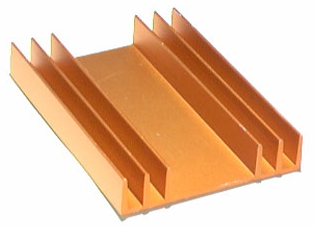
\includegraphics[scale=1]{figuras/10b-6225M-ZD-5.png}
\caption{Disipador comercial 6225M ZD-5, Rda=5,1$\dfrac{^{o}C}{W}$}
\label{figura10b}
\end{figure}

\subsubsection{Punto 10.c)}
\textbf{Enunciado : } Comparar con los disipadores utilizados originalmente por Turner y obtener conclusiones\\[1cm]

\subsection{Punto 11}
\textbf{Simular el comportamiento estático y dinámico del amplificador determinando:}\\

\subsubsection{Punto 11.a)}
\textbf{Enunciado : } Medir las tensiones de todos los nodos y las corrientes de todas las ramas para VG=0V\\[1cm]
\begin{figure}[H]
\centering
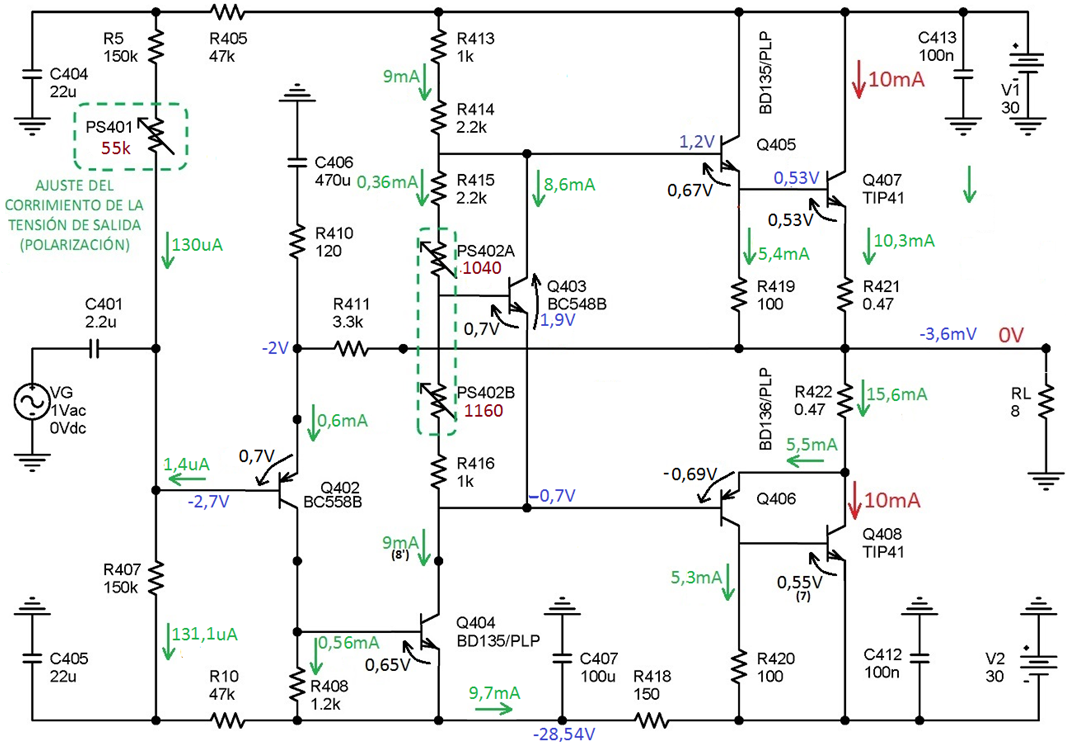
\includegraphics[scale=0.4]{figuras/11-a-valoresReposo.png}
\caption{Valores obtenidos de la simulación del punto de operación}
\label{figura11a}
\end{figure}
Vemos una gran similitud con los valores calculados anteriormente, Fig.\eqref{figura1}, aunque hubo que cambiar PS401 con respecto al calculado para acercarnos lo más posible a 0V en la salida, y tambíén PS402A y PS402B para asegurar 10mA en los colectores de Q407 y Q408.

\subsubsection{Punto 11.b)}
\textbf{Enunciado : } Medir la impedancia de entrada en función de la frecuencia (desde 0,1Hz hasta 1GHz)\\[1cm]
\begin{figure}[H]
\centering
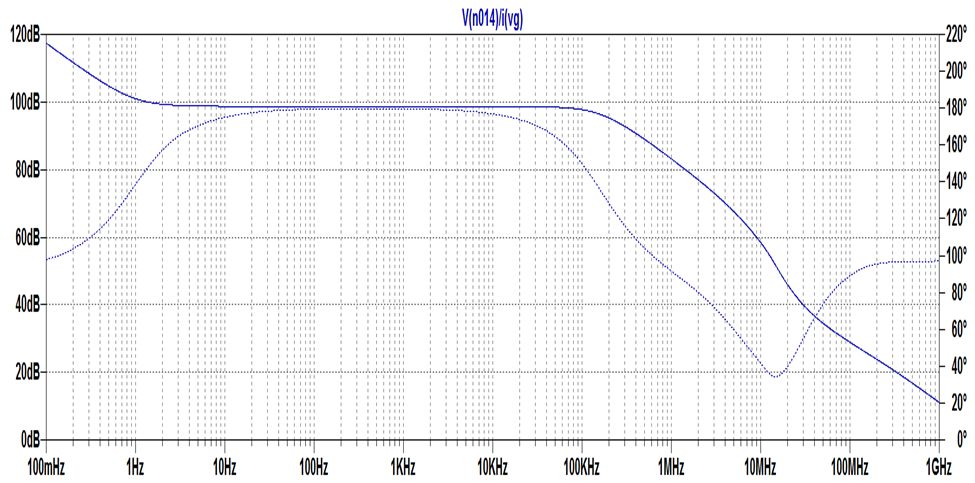
\includegraphics[scale=0.4]{figuras/11-b-Zin.png}
\caption{Impedancia de entrada en función de la frecuencia}
\label{figura11b}
\end{figure}
\begin{center}
Rin(1KHz) = $10^\frac{98,7}{20}\Omega$ = 86023,2$\Omega$
\end{center}
Recordemos que el valor calculado fue :\quad Rin=85K$\Omega$

\subsubsection{Punto 11.c)}
\textbf{Enunciado : } Medir la impedancia de salida en función de la frecuencia (desde 0,1Hz hasta 1GHz)\\[1cm]
\begin{figure}[H]
\centering
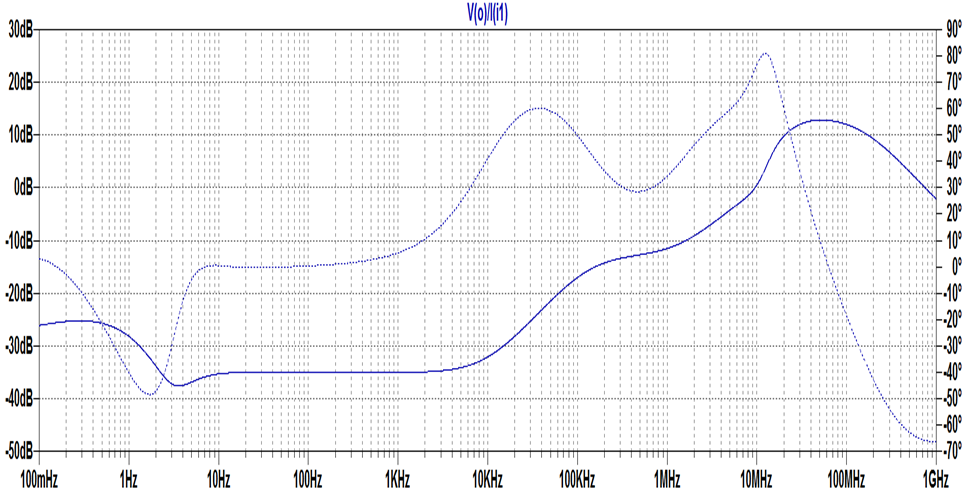
\includegraphics[scale=0.4]{figuras/11-c-Zout.png}
\caption{Impedancia de salida en función de la frecuencia}
\label{figura11c}
\end{figure}
\begin{center}
Ro(1KHz) = $10^\frac{-35.08}{20}\Omega$ = 17,6m$\Omega$
\end{center}
Recordemos que el valor calculado fue :\quad Ro=12,9m$\Omega$

\subsubsection{Punto 11.d)}
\textbf{Enunciado : } Respuesta en frecuencia para 1W sobre la carga)\\[1cm]
Tenemos : $Po=\dfrac{(Vo_{ef})^2}{RL}=\dfrac{(Vop)^2}{2\:RL}=1W$ \quad con Vop=Vo pico\\
Vop = $\sqrt{Po\:\:2\:RL}$ = 4V\quad $\Longrightarrow$\qquad Vip= $\dfrac{Vop}{A}$ = $\dfrac{4V}{28,3}$ = 141mV
\begin{figure}[H]
\centering
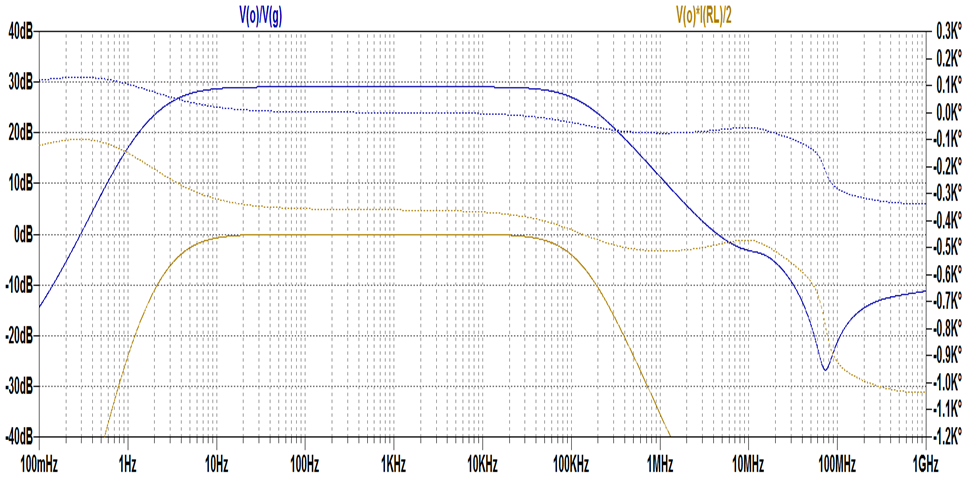
\includegraphics[scale=0.4]{figuras/11-d-Pcarga1W.png}
\caption{Respuesta en frecuencia para 1W sobre la carga}
\label{figura11d}
\end{figure}
\begin{center}
\textcolor{blue}{A(1KHz) = 29dB}\qquad $\Longrightarrow$\qquad A=28,2\\
\textcolor{orange}{Po(1KHz) = 0dB}\qquad $\Longrightarrow$\qquad Po=1W
\end{center}
$f_{h}(-3dB)$=83,17KHz\qquad $f_{l}(-3dB)$=4,7Hz
\begin{center}
BW = $f_{h}-f_{l}$ = 83,17KHz
\end{center}

\subsubsection{Punto 11.e)}
\textbf{Enunciado : } Ancho de banda de potencia\\
Es la máxima frecuencia para la que el amplificador logra reproducir una señal sinusoidal a máxima potencia (hallada en el punto 4 sin deformación)\\[1cm]
Vop = $\sqrt{Po\:\:2\:RL}$ = 21,3V\qquad $\Longrightarrow$\qquad Vip= $\dfrac{Vop}{A}$ = $\dfrac{21,3V}{28,3}$ = 752mV
\begin{figure}[H]
\centering
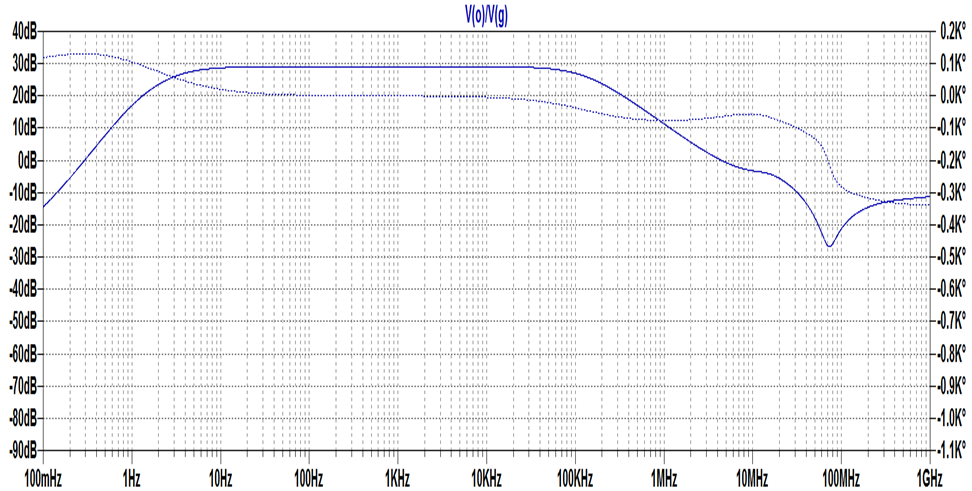
\includegraphics[scale=0.4]{figuras/11-e-BWdePot.png}
\caption{Ancho de banda de potencia}
\label{figura11e}
\end{figure}
Como se trata de gran señal se harán simulaciones en tiempo en lugar de frecuencia.\\
Subjetivamente se ve que a partir de 42KHz distorsiona, pero objetivamente?

\subsubsection{Punto 11.f)}
\textbf{Enunciado : } Respuesta al escalón\\
\begin{itemize}

\item i. Pequeña señal (la tensión pico de salida estará entre 0,1V y 1V)
\end{itemize}
Usando una tensión de entrada $V_{in}=\dfrac{1V}{A}=35mV$, donde A es la ganancia del sistema realimentado, obtenemos :
\begin{figure}[H]
\centering
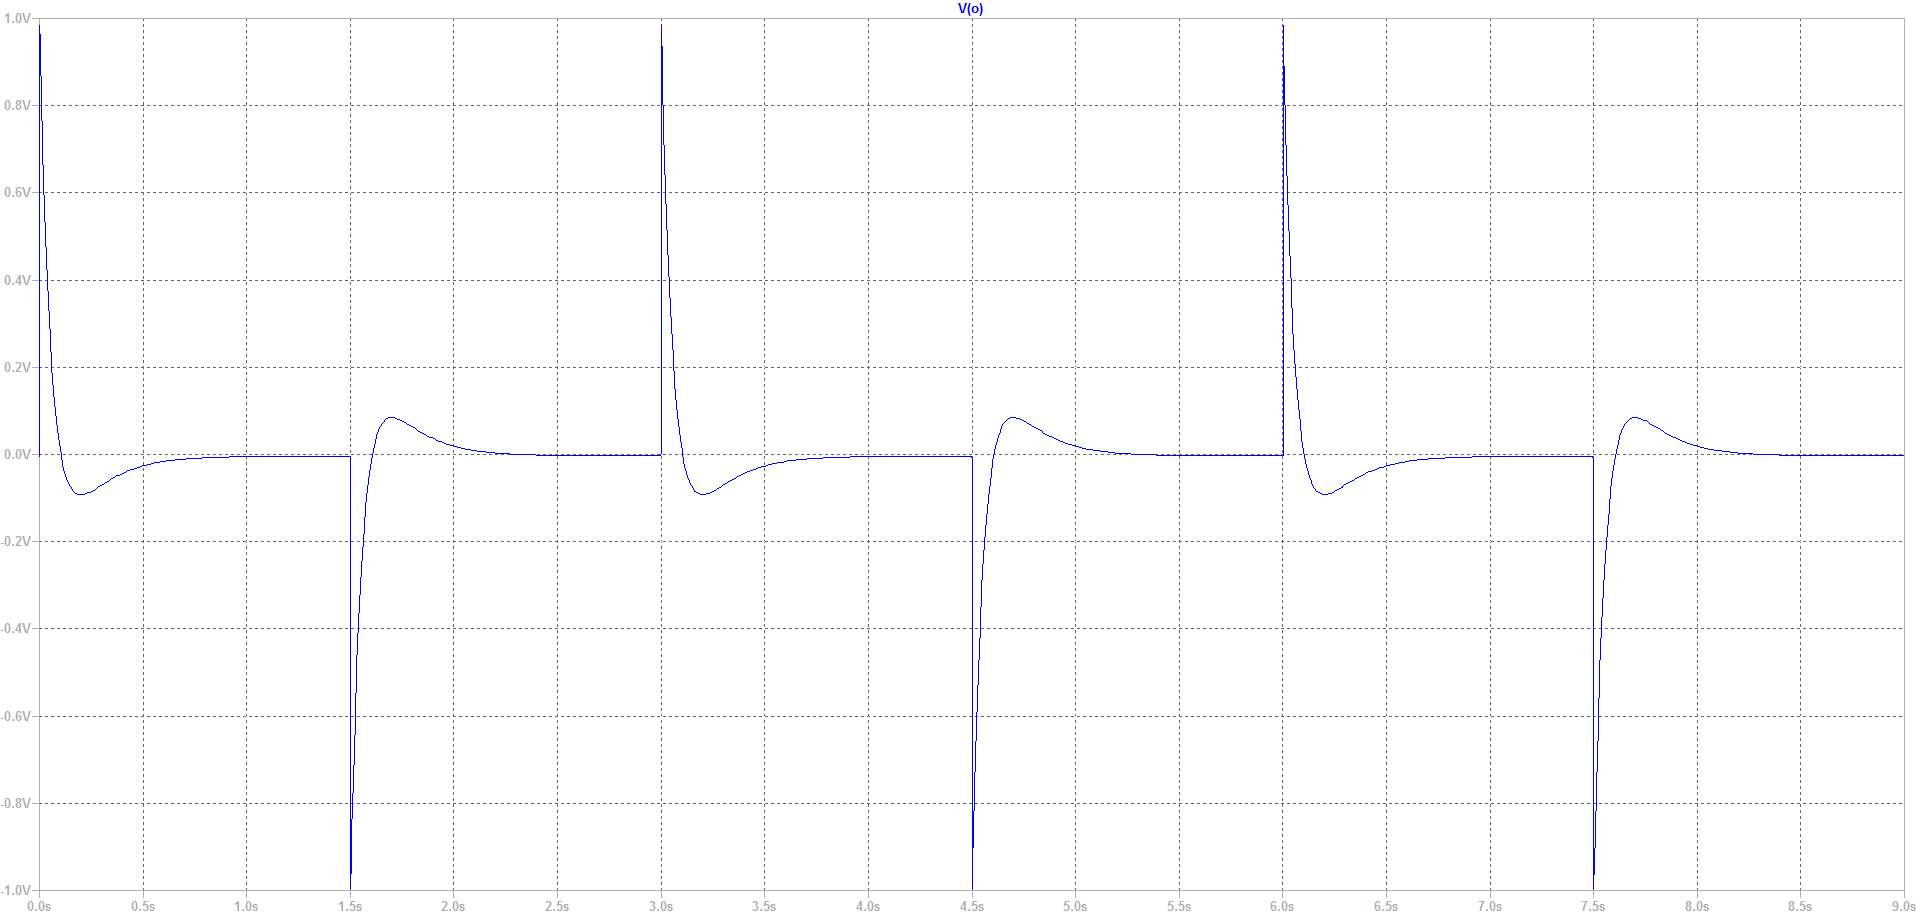
\includegraphics[scale=0.2]{figuras/11-f-i-escalon.png}
\caption{Respuesta al escalón, pequeña señal.}
\label{figura11fi}
\end{figure}

\begin{itemize}
\item ii. Gran señal (amplitud de salida apenas menor que la máxima tensión pico de salida hallada en el punto 8
\end{itemize}
\begin{figure}[H]
\centering
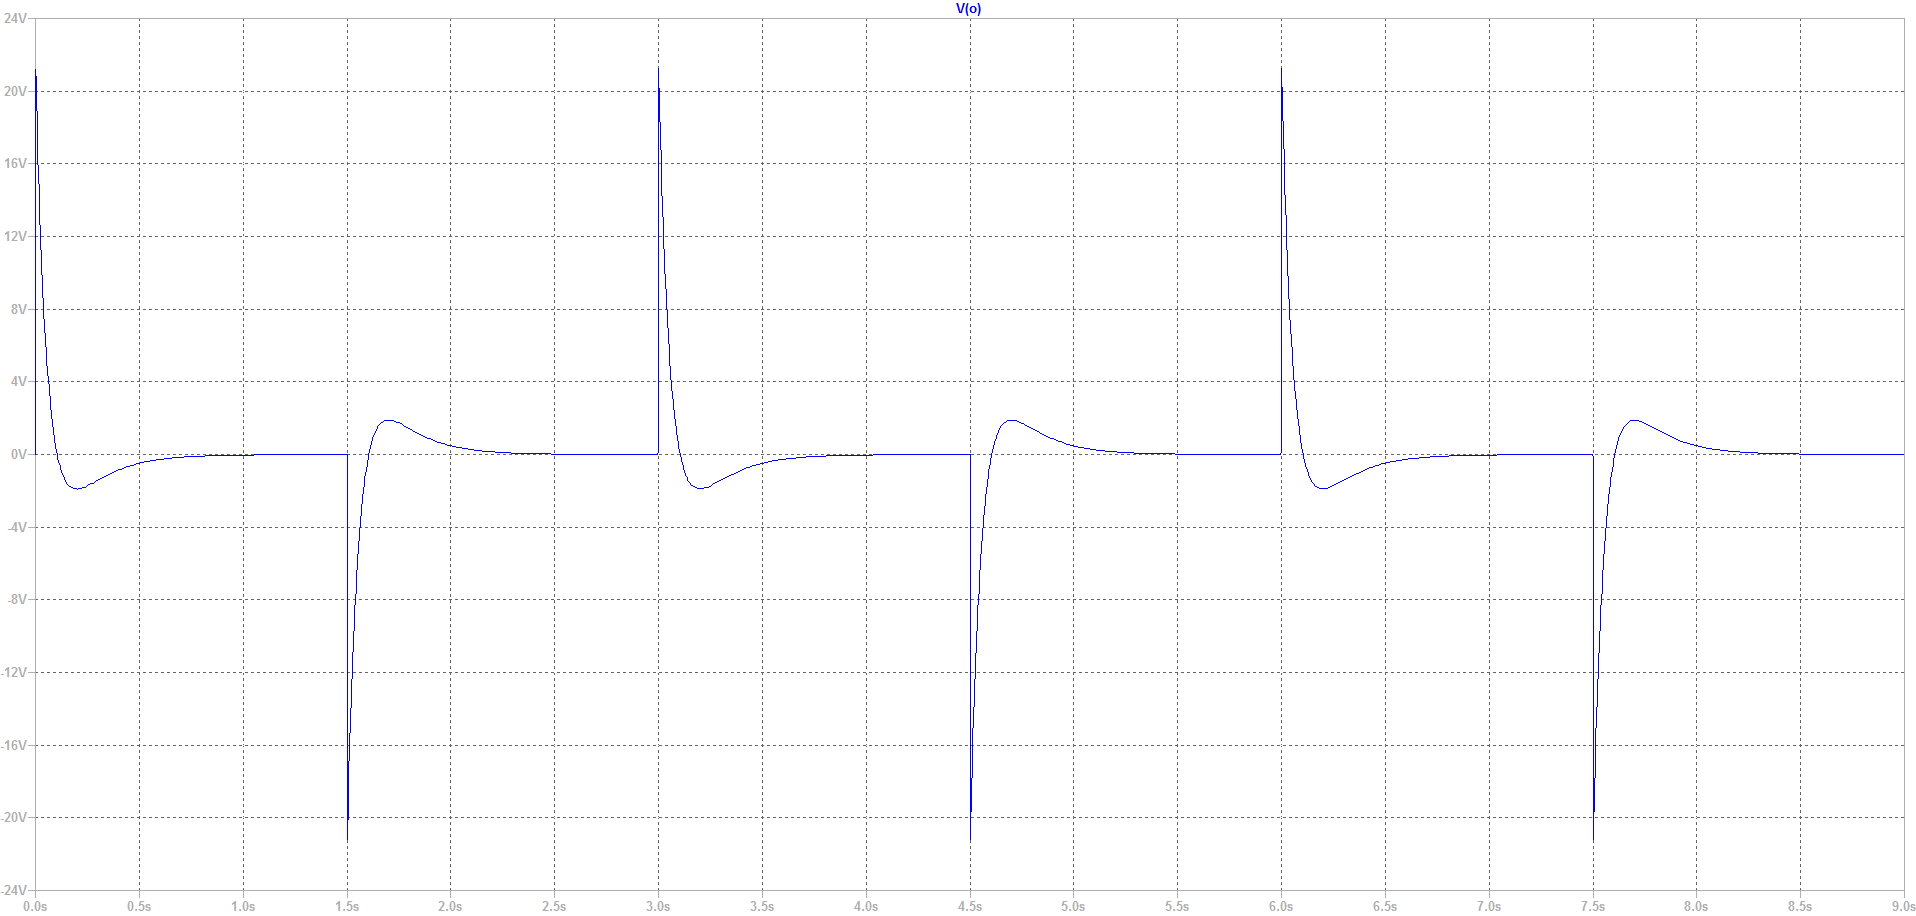
\includegraphics[scale=0.2]{figuras/11-f-ii-escalon2.png}
\caption{Respuesta al escalón, gran señal.}
\label{figura11fii}
\end{figure}

\begin{itemize}
\item iii. En base a lo medido en i.determinar el ancho de banda para pequeña señal asumiendo que el amplificador está compensado por polo dominante
\end{itemize}

\begin{itemize}
\item iv. En base a lo medido en ii.determinar la velocidad de crecimiento de la tensión de salida (“slewrate”)
\end{itemize}

\subsubsection{Punto 11.g)}
\textbf{Enunciado : } Determinar el margen de fase\\[1cm]
A partir de la siguiente figura observamos el margen de fase que le queda a la ganancia de lazo, T, para alcanzar los $180^o$.
\begin{figure}[H]
\centering
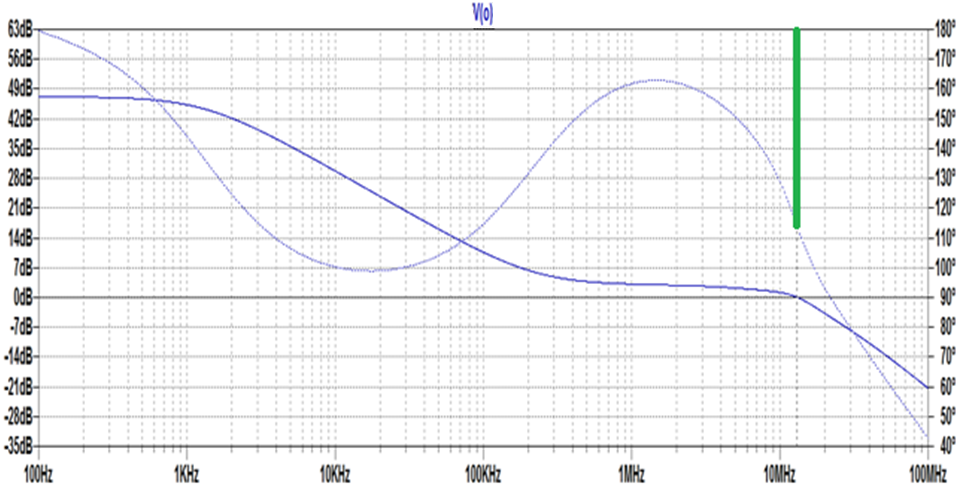
\includegraphics[scale=0.4]{figuras/11-g-margenFase.png}
\caption{Margen de fase, MF.}
\label{figura11g}
\end{figure}
\begin{center}
Margen de fase :\quad MF $=180^{o}-114^{o}=66^{o}$
\end{center}
Observamos que el módulo de T a frecuencias medias es de 47dB, cercano a los 44,3dB calculados en el punto 2.

\subsubsection{Punto 11.h)}
\textbf{Enunciado : } Determinar la distorsión armónica a 1KHz y a 10KHz para potencias de 0,1W; 1W; 10W y 90\% de la máxima calculada en el punto 4\\[1cm]
Primeramente obtenemos la tensión de entrada $v_i$ necesaria para obtener esos valores de potencia de salida.\\
Siendo $Vo_{pico}=\sqrt{Po\:\:2\:RL}$\, y\, $Vi_{pico}=\dfrac{Vo_{pico}}{A}$, tenemos :
\begin{table}[H]
\centering
\begin{tabular}{|c|c|c|}
\hline
Po[W]&$Vo_{pico}$[V]&$Vi_{pico}$[mV]\\
\hline
0,1&1,26&44,7\\
\hline
1&4&141,3\\
\hline
10&12,65&447\\
\hline
25,65&20,26&715,8\\
\hline
\end{tabular}
\caption{Valores de $v_i$ para obtener la distorsión armónica}
\label{Vi-distorsion}
\end{table}

Usando los comandos SPICE :
\begin{itemize}
\item .FOUR 1K 10 -1 V(o)
\item .FOUR 10K 10 -1 V(o)
\end{itemize}
Para obtener la distorsión armónica total (THD)de las 10 primeras armónicas en la tensión de salida Vo cuando la frecuencia de entrada es de 1KHz y 10KHz respectivamente.\\
Se tomarán los 10 primeros períodos en ambos casos, el ``-1'' es para que realice el análisis sobre todo el tiempo simulado, 10ms para 1KHz y 1ms para 10KHz, obtuvimos :\\
\begin{table}[H]
\centering
\begin{tabular}{|c|c|c|}
\hline
Po[W]&THD[\%] (1KHz)&THD[\%] (10KHz)\\
\hline
0,1&0,046&0,157\\
\hline
1&0,039&0,094\\
\hline
10&0,011&0,065\\
\hline
25,65&0,038&0,086\\
\hline
\end{tabular}
\caption{Distorsión armónica total para frecuencias de entrada 1KHz y 10KHz.}
\label{11h-THD}
\end{table}
Vemos que la distorsión es menor para 1KHz de frecuencia de entrada y también que presenta un mínimo alrededor de la potencias medias, es decir, disminuye de bajas a medias potencias y sube de medias a altas potencias.

\subsubsection{Punto 11.i)}
\textbf{Enunciado : } Determinar la distorsión por intermodulación para potencias de 0,1W; 1W; 10W y 90\% de la máxima calculada en el punto 4\\[1cm]

\subsubsection{Punto 11.j)}
\textbf{Enunciado : } Determinar el Rechazo de Ruido de la Fuente de Alimentación (“PSNR”)\\[1cm]
Se pasivó la señal de entrada y se agregó a cada fuente de alimentación una fuente de prueba Vp.\\
Obteniendo el rechazo de ruido de la fuente de alimentación como:
\begin{center}
PSNR=$\dfrac{Vo_{pico}}{Vp_{pico}}$
\end{center}
Se simuló para las frecuencias 50Hz, 100Hz, 1KHz, 10KHz, 50KHz y 100KHz con una $Vp_{pico}$ de 1mV.\\
Se obtuvo :
\begin{center}
\begin{tabular}{llllll}
-54dB&-60dB&-80dB&-95dB&-91dB&-86dB\\
0,2\%&0,1\%&0,01\%&0,018\%&0,027\%&0,051\%\\
\end{tabular}
\end{center}
respectivamente.\\
Se observa que varia con la frecuencia, con un mínimo a 10KHz. En la frecuencia de alimentación de red (50Hz) vemos una atenuación aceptable, en la salida se observa el ruido de esa fuente atenuado 500 veces. Al variar $Vp_{pico}$ alrededor de 1mV no se observaron cambios.

\end{document}